\chapter{Implementação do Processo}

A execução do processo ocorre por meio de componentes para a análise de similaridade, persistência dos dados, geração do alinhamento, lógica entre as etapas e utilitários para manipulação de dados (ver Figura \ref{fig:componentes}). Alguns componentes foram reusados, como o de similaridade léxica, que contém vários algoritmos para detectar a similaridade entre textos. Outros componentes foram desenvolvidos, como os responsáveis pela detecção da similaridade de recurso, alinhamento e outros.

\begin{figure}[!ht]
	\centering
	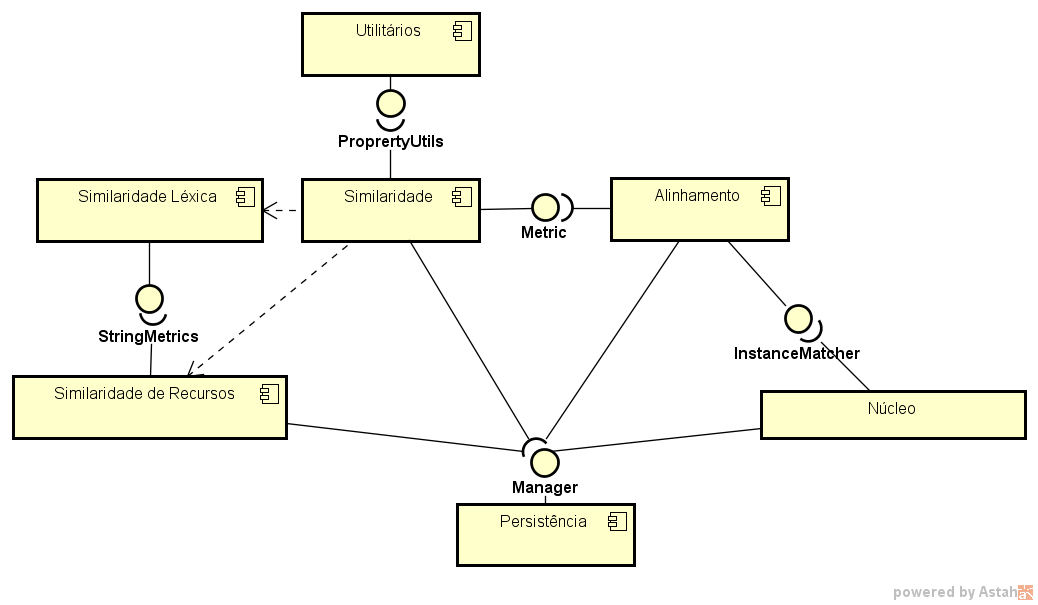
\includegraphics[width=0.9\textwidth]{./imagens/componentes.png}
    \caption{Componentes utilizados na implementação do processo}
	\label{fig:componentes}
\end{figure}

Apesar de existirem diversas soluções que contém algoritmos para o cálculo de similaridade e alinhamento entre recursos, optou-se pelo desenvolvimento de uma abordagem que contemplasse problemas provenientes de bases de dados reais (acentuação, ausência de propriedades, formatação e outros).
Os principais componentes utilizados são:

\section*{Persistência}
O componente de persistência é responsável pelo acesso à base de conhecimento. Assim, é responsável por armazenar e recuperar os recursos e os alinhamentos que são utilizados ao longo do processo. Além disso, o mesmo atua como abstração do servidor de triplas (Virtuoso, OWLim etc.).

\section*{Similaridade}
O componente de similaridade é dividido em dois subcomponentes, sendo eles o de similaridade léxica e recurso. O primeiro utiliza métricas como distância de Levenshtein \cite{levenshtein1966binary}, Cosseno \cite{singhal2001modern}, Jaro-Winkler \cite{winkler1990string} e outros. O segundo componente, que se refere à similaridade de recurso, utiliza o primeiro e tem como função gerar a similaridade entre recursos.

Para a cálculo da similaridade dos recursos foi utilizada uma abordagem baseada na técnica de subgrafo semântico, tal abordagem foi utilizada com o intuito de reduzir o nível de incerteza. Nesta abordagem é gerado um subgrafo com o recurso seus recursos relacionados. Além disso, é importante destacar que a semântica das relações entre os elementos é levada em consideração, de forma que apenas propriedades de semântica equivalente são comparados.

Para definir a similaridade de recurso formalmente foram usadas duas equações. A Equação \ref{eq:properties_definition} define o conjunto de propriedades que será considerado durante a comparação entre os recursos, onde esse é igual a subtração entre maior conjunto de propriedades e o conjunto de propriedades que deve ser desconsiderado. Logo:

\begin{equation}
P_f =M a x  ( P_{r f} ,P_{r o} ) - P_d
\label{eq:properties_definition}
\end{equation}

Onde:
\begin{itemize}
	\item $P_{r f}$ – Propriedades do recurso fonte;
	\item $P_{r o}$ –  Propriedades do recurso objeto;
	\item $P_d$ –  Propriedades a ser desconsideradas;
	\item $M a x  ( P_{r f} ,P_{r o} )$ – Retorna o maior conjunto de propriedades;
\end{itemize}

A Equação \ref{eq:similaridade} trata da função de similaridade entre recursos, essa equação pode ser entendida como a média das similaridades entre dois recursos.

\begin{equation}
SR  = \frac{1}{|P_f|} { \sum_{i = 1}^{P_f} {S(V(R1,P_f[i]);V(R2,P_f[i]))}}
\label{eq:similaridade}
\end{equation}

Onde:

\begin{itemize}
	\item S – Função de similaridade léxica;
	\item V(R,P) – Valor da propriedade P em um recurso R;
	\item R1 – Recurso 1;
	\item R2 – Recurso 2;
\end{itemize}

O valor gerado pelo componente de similaridade é enviado para o componente de alinhamento.


\section*{Alinhamento}
O componente de alinhamento tem como responsabilidade determinar, de acordo com os valores obtidos na etapa de similaridade, se os recursos analisados realmente dizem respeito à mesma entidade do mundo real. Para determinar se o alinhamento deve ser realizado, este componente faz uso de limiares de aceitação, que são determinados previamente. Por esse motivo, o processo de alinhamento não é uma tarefa automática, pois precisa que os valores sejam ajustados.

Os valores de similaridade são comparados com o limiar, caso o valor esteja em uma faixa aceitável, será realizado o alinhamento entre os respectivos recursos, em caso contrário o alinhamento não será persistido. Assim como os componentes principais, os componentes auxiliares têm suas respectivas funções. De modo geral, esses componentes devem auxiliar os componentes principais. Tais componentes serão descritos a seguir.


\section*{Núcleo}
O componente de núcleo tem como principal função coordenar as atividades de alinhamento. Além de coordenar, é nesse componente que são definidos os limiares de aceitação, propriedades a serem desconsideradas, conceitos principais e conceitos relacionados, que servirão como parâmetro os componentes de alinhamento e similaridade.


\section*{Utilitários}
O componente de utilitários tem como função realizar tratamentos nos textos que serão aplicados à função de similaridade. Alguns exemplos de tratamento são: tratamento de acentos, pontuação e outros.

